\section{Theorie}
\label{sec:Theorie}
In diesem Versuch sollen die charakteristischen Eigenschaften von Strömungen mit dem Impuls-Echo-Verfahren untersucht werden.\\
Der Doppler-Effekt tritt auf, wenn sich ein Beobachter und eine Schallquelle relativ zueinander bewegen und es zu einer Änderung der Frequenz kommt.
Bewegt sich die Quelle auf den Beobachter zu, verschiebt sich die Frequenz $\nu_0$ zu höheren Frequenzen $\nu_\text{kl}$. Entfernt sich die Quelle vom Beobachter sinkt die Frequenz $\nu_\text{gr}$ nach
\begin{equation}
    \nu_\text{kl/gr}=\frac{\nu_0}{1\mp \frac{v}{c}} \, .
\end{equation}
Dabei ist $v$ die Geschwindigkeit und $c$ die Schallgeschwindigkeit.
Bei ruhender Quelle und auf die Quelle zu bewegtem Beobachter verschiebt sich die Frequenz in höhere Fequenzen $\nu_\text{h}$.
Entfernt sich der Beobachter veringert sich die Frequenz zu $\nu_\text{n}$ nach 
\begin{equation}
    \nu_\text{h/n}= \nu_0 \left(1 \pm \frac{v}{c}\right) \, .
\end{equation}
Der Doppler-Effekt kann im Bereich der Ultraschalltechnik verwendet werden um z.B. die Geschwindigkeit von Blutströmungen zu bestimmen. 
\begin{figure}
    \centering
    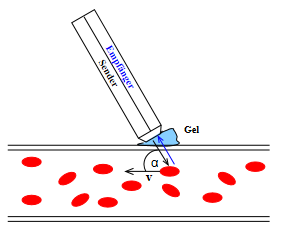
\includegraphics[scale=0.4]{pics/Blut.png}
    \caption{Darstellung des Impuls-Echo-Verfahren \cite{v903}}
    \label{fig:IEV}
  \end{figure}
Dabei tritt der Doppler-Effekt auf wenn eine Ultraschallwelle auf ein bewegtes Objekt trifft, wie in Abbildung \ref{fig:IEV} zu sehen. Die Frequenzverschiebung 
\begin{equation}
    \symup{\Delta}\nu=\nu_0 \frac{v}{c}\left(\cos \alpha + \cos \beta \right)
\end{equation}
wird neben der Geschwindigkeit $v$ und der Schallgeschwindigkeit $c$ durch die Winkel $\alpha$ und $\beta$ bestimmt. Bei dem verwendeteten Impuls-Echo-Verfahren sind die Winkel $\alpha$ und $\beta$ identisch,
sodass sich für die Geschwindigkeit $v$
\begin{equation}
    v= \frac{\symup{\Delta}\nu c}{2 \nu_0 \cos \alpha}
    \label{eqn:geschw}
\end{equation}
ergibt. Dabei ist $\alpha$ der Winkel zwischen der Geschwindigkeit und der Wellennormalen der einlaufenden Welle. Schallwellen können auf verschiedene Arten erzeugt werden.
Eine Methode ist die Ausnutzung des piezo-elektrischen Effekts. Dabei wird ein Piezoelektrischer Kristall in einem elektrischem Wechselfeld in Schwingung angeregt.
Beim Schwingen strahlt der Kristall Ultraschallwellen ab. Es können große Schwingungsamplituden erreicht werden, sodaß extrem hohe Schallwellendichten genutzt werden können, wenn es zu Resonanz kommt.
Der Piezokristall kann auch als Empfänger von Scahllwellen genutzt werden.
